\begin{frame}
  \frametitle{Fact 1 -- Sum of Degrees}
{ \Huge
  \[
    \sum_{u\in V} degree(u) = 2|E|
  \]
}
  Every edge contributes exactly once to the degree of exactly two nodes.
\end{frame}

\begin{frame}
  \frametitle{Fact 2 -- Average Degree}
\begin{equation}
\begin{aligned}
E(degree(X)) & = \sum_{u\in V} Pr(X=u)\cdot degree(u)\\
              & = \frac{1}{n} \sum_u degree(u) = \frac{2|E|}{n}
  \end{aligned}
  \end{equation}
\end{frame}

\begin{frame}
  \frametitle{Fact 3 -- Min-cut Size}

  The size of a min-cut is at most $\frac{2|E|}{n}$.

  \only<1>{ 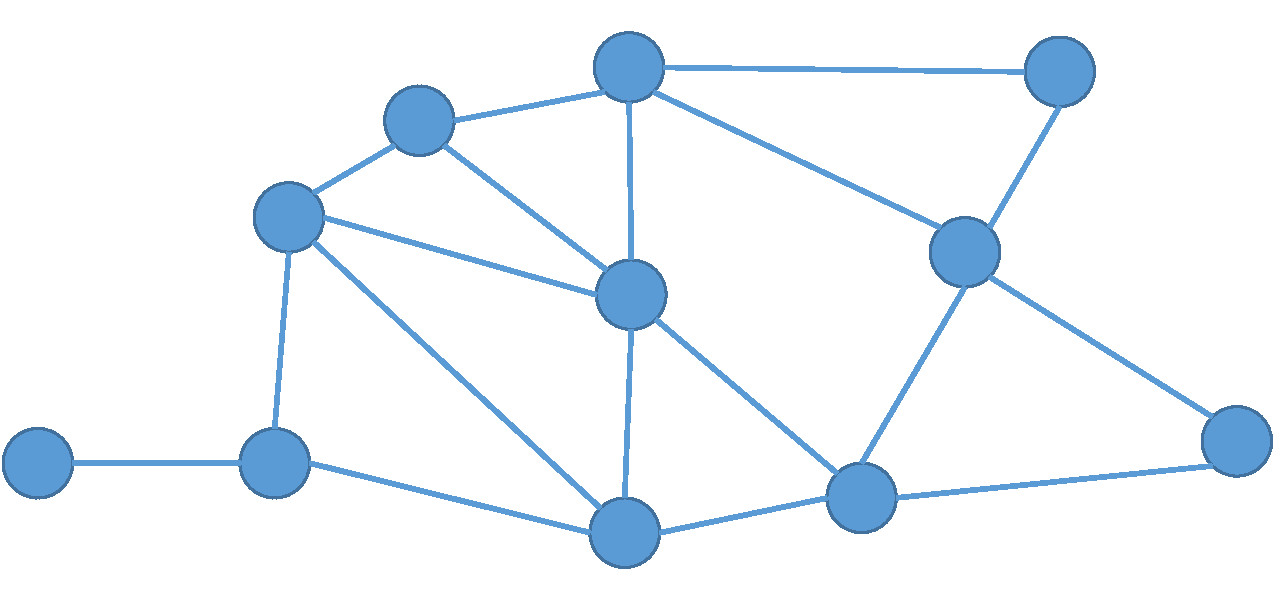
\includegraphics[scale=0.4]{img/fact3_1.pdf} }
  \only<2>{ 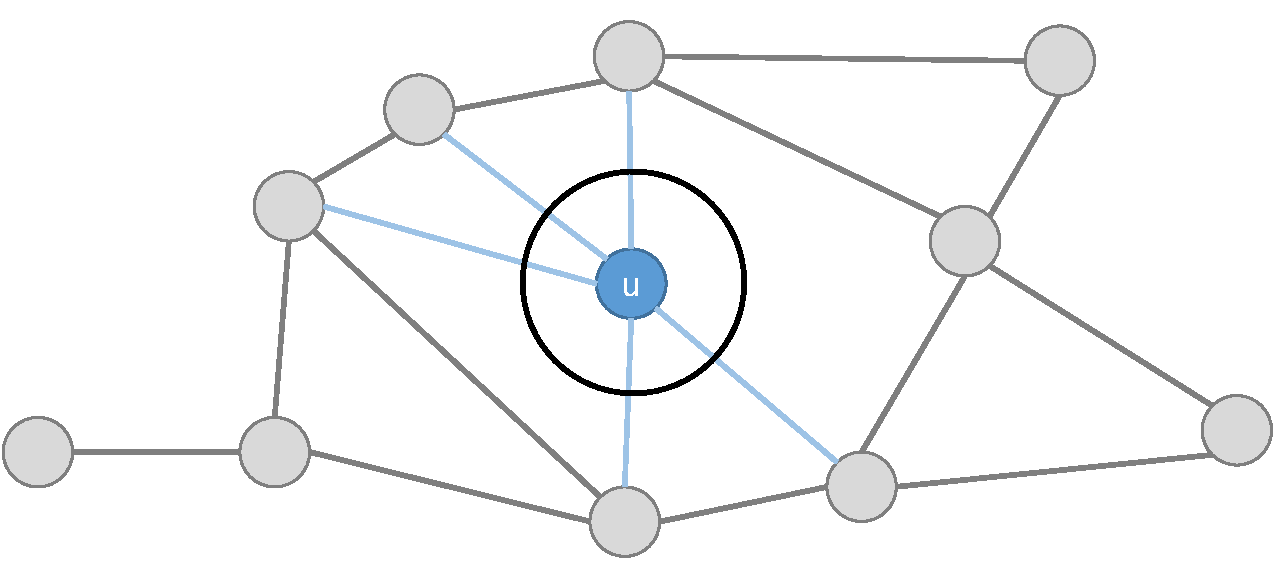
\includegraphics[scale=0.4]{img/fact3_2.pdf} }
  \only<3>{
    \begin{greenblock}{Proof}
      \begin{itemize}
        \item For every node $u$, we have a cut of size $degree(u)$.
        \item Not all nodes can have degree above average, i.e.
      \end{itemize}
      \[
        \exists u\in V:\ degree(u) \leq \frac{2|E|}{n}
      \]
    \end{greenblock}
  }

\end{frame}

\begin{frame}
  \frametitle{Fact 4 -- Pr(edge across min-cut)}

  \begin{itemize}
    \item Fix a certain min-cut in a graph.
    \item At most $2|E|/n$ of all edges are part of this min-cut.
    \item Choose a random edge out of all $|E|$ edges.
    \item $Pr(\text{edge crosses the cut}) = \frac{2|E|/n}{|E|} = \frac{2}{n}$
  \end{itemize}

\end{frame}
